\section{Results}
\label{sec:results}

\subsection{Discrimination and calibration}
Tables~\ref{tab:readmit} and~\ref{tab:esc} and Fig.~\ref{fig:auroc} report
test performance. For 30-day readmission under the patient-grouped design,
TKGN-B reached a mean AUROC of \AucReadmitGrpTKGNB{}
($\pm$\AucSdReadmitGrpTKGNB{}) and AUPRC of \PrcReadmitGrpTKGNB{}, the
highest of all models, followed closely by XGBoost (\AucReadmitGrpXGB{}) and
LightGBM (\AucReadmitGrpLGBM{}). The three sequence baselines were tightly
grouped (GRU \AucReadmitGrpGRU{}, RETAIN \AucReadmitGrpRETAIN{},
Transformer \AucReadmitGrpTRF{}), and TKGN on its own matched them
(\AucReadmitGrpTKGN{}) without surpassing the boosting models. Logistic
regression (\AucReadmitGrpLR{}) and the multilayer perceptron
(\AucReadmitGrpMLP{}) were clearly weaker. For treatment escalation the
ranking was similar: TKGN-B \AucEscGrpTKGNB{} ($\pm$\AucSdEscGrpTKGNB{}),
LightGBM \AucEscGrpLGBM{}, XGBoost \AucEscGrpXGB{}, random forest
\AucEscGrpRF{}, sequence models between \AucEscGrpRETAIN{} and
\AucEscGrpGRU{}, and TKGN \AucEscGrpTKGN{}. The absolute level of
discrimination is modest for both tasks, in line with the range usually
reported for readmission \citep{kansagara2011}.

\begin{table*}[t]
  \centering
  \caption{Test performance for 30-day readmission. Grouped split: mean$\pm$SD
  over five patient-disjoint repeats; temporal split: mean over three seeds.
  Slope: calibration slope; Sens./Spec.: at the validation-selected
  threshold. Best AUROC per design in bold.}
  \label{tab:readmit}
  \scriptsize
  \setlength{\tabcolsep}{3.2pt}
  \begin{tabular}{@{}lccccccc|cc@{}}
\toprule
 & \multicolumn{7}{c|}{Patient-grouped split (5 repeats, mean$\pm$SD)} & \multicolumn{2}{c}{Temporal split} \\
Model & AUROC & AUPRC & Brier & ECE & Slope & Sens. & Spec. & AUROC & AUPRC \\
\midrule
Logistic regression & 0.669$\pm$0.005 & 0.223$\pm$0.007 & 0.096$\pm$0.001 & 0.006$\pm$0.001 & 0.85 & 0.41 & 0.81 & 0.603 & 0.190 \\
Random forest & 0.682$\pm$0.005 & 0.233$\pm$0.011 & 0.096$\pm$0.001 & 0.008$\pm$0.001 & 1.20 & 0.39 & 0.84 & \textbf{0.700} & 0.238 \\
XGBoost & 0.688$\pm$0.004 & 0.247$\pm$0.006 & 0.095$\pm$0.001 & 0.004$\pm$0.002 & 1.04 & 0.41 & 0.83 & 0.684 & 0.234 \\
LightGBM & 0.688$\pm$0.004 & 0.247$\pm$0.007 & 0.095$\pm$0.001 & 0.004$\pm$0.002 & 1.04 & 0.38 & 0.85 & 0.685 & 0.234 \\
MLP & 0.653$\pm$0.009 & 0.212$\pm$0.009 & 0.097$\pm$0.001 & 0.017$\pm$0.006 & 0.69 & 0.42 & 0.78 & 0.601 & 0.187 \\
\midrule
GRU & 0.682$\pm$0.005 & 0.236$\pm$0.010 & 0.095$\pm$0.001 & 0.011$\pm$0.002 & 0.99 & 0.41 & 0.82 & 0.684 & 0.228 \\
RETAIN & 0.683$\pm$0.006 & 0.237$\pm$0.010 & 0.096$\pm$0.001 & 0.015$\pm$0.004 & 0.95 & 0.44 & 0.80 & 0.687 & 0.229 \\
Transformer & 0.683$\pm$0.006 & 0.237$\pm$0.013 & 0.096$\pm$0.001 & 0.015$\pm$0.008 & 0.86 & 0.41 & 0.82 & 0.690 & 0.231 \\
\midrule
TKGN (proposed) & 0.682$\pm$0.004 & 0.238$\pm$0.011 & 0.095$\pm$0.001 & 0.014$\pm$0.007 & 0.90 & 0.41 & 0.82 & 0.689 & 0.236 \\
TKGN-B (proposed) & \textbf{0.690$\pm$0.005} & 0.250$\pm$0.009 & 0.095$\pm$0.001 & 0.007$\pm$0.004 & 0.89 & 0.41 & 0.83 & 0.685 & 0.235 \\
\bottomrule
\end{tabular}

\end{table*}

\begin{table*}[t]
  \centering
  \caption{Test performance for treatment escalation at the next stay
  (same layout as Table~\ref{tab:readmit}).}
  \label{tab:esc}
  \scriptsize
  \setlength{\tabcolsep}{3.2pt}
  \begin{tabular}{@{}lccccccc|cc@{}}
\toprule
 & \multicolumn{7}{c|}{Patient-grouped split (5 repeats, mean$\pm$SD)} & \multicolumn{2}{c}{Temporal split} \\
Model & AUROC & AUPRC & Brier & ECE & Slope & Sens. & Spec. & AUROC & AUPRC \\
\midrule
Logistic regression & 0.666$\pm$0.013 & 0.506$\pm$0.007 & 0.211$\pm$0.003 & 0.018$\pm$0.004 & 0.85 & 0.82 & 0.37 & 0.646 & 0.497 \\
Random forest & 0.685$\pm$0.012 & 0.531$\pm$0.010 & 0.208$\pm$0.003 & 0.034$\pm$0.006 & 1.46 & 0.78 & 0.47 & 0.671 & 0.514 \\
XGBoost & 0.687$\pm$0.013 & 0.535$\pm$0.010 & 0.205$\pm$0.003 & 0.015$\pm$0.005 & 1.07 & 0.81 & 0.42 & 0.673 & 0.519 \\
LightGBM & 0.687$\pm$0.012 & 0.536$\pm$0.012 & 0.205$\pm$0.003 & 0.014$\pm$0.008 & 1.07 & 0.80 & 0.45 & 0.673 & 0.516 \\
MLP & 0.646$\pm$0.007 & 0.485$\pm$0.004 & 0.217$\pm$0.002 & 0.046$\pm$0.010 & 0.62 & 0.77 & 0.42 & 0.622 & 0.467 \\
\midrule
GRU & 0.681$\pm$0.014 & 0.527$\pm$0.014 & 0.208$\pm$0.004 & 0.032$\pm$0.011 & 0.86 & 0.79 & 0.44 & 0.670 & 0.516 \\
RETAIN & 0.677$\pm$0.013 & 0.517$\pm$0.015 & 0.209$\pm$0.004 & 0.034$\pm$0.011 & 0.85 & 0.75 & 0.50 & 0.668 & 0.518 \\
Transformer & 0.679$\pm$0.013 & 0.526$\pm$0.010 & 0.209$\pm$0.005 & 0.040$\pm$0.015 & 0.76 & 0.78 & 0.46 & 0.668 & 0.516 \\
\midrule
TKGN (proposed) & 0.678$\pm$0.012 & 0.525$\pm$0.009 & 0.209$\pm$0.005 & 0.035$\pm$0.017 & 0.82 & 0.77 & 0.47 & 0.668 & 0.514 \\
TKGN-B (proposed) & \textbf{0.688$\pm$0.013} & 0.537$\pm$0.011 & 0.205$\pm$0.004 & 0.016$\pm$0.006 & 0.99 & 0.76 & 0.49 & \textbf{0.680} & 0.525 \\
\bottomrule
\end{tabular}

\end{table*}

\begin{figure*}[t]
  \centering
  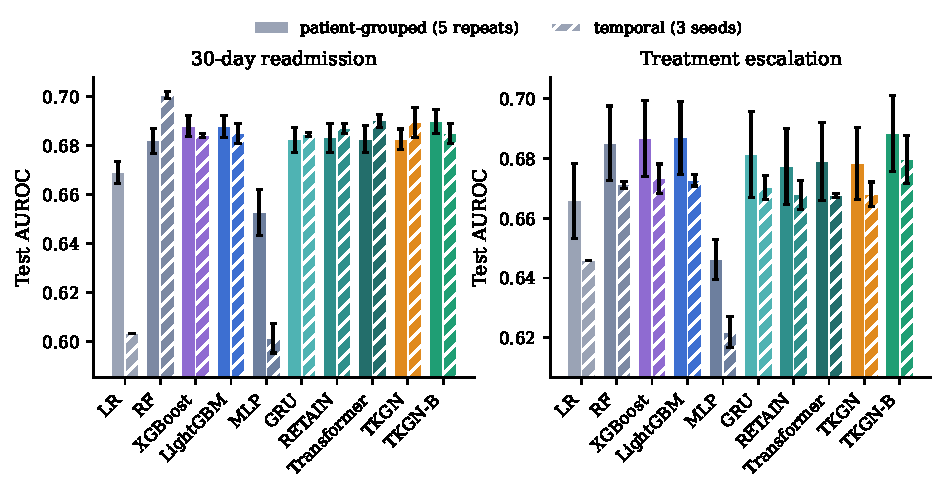
\includegraphics[width=\textwidth]{figures/fig_auroc.pdf}
  \caption{Test AUROC of all models. Solid bars: patient-grouped split
  (mean$\pm$SD over five repeats); hatched bars: temporal split (mean$\pm$SD
  over three seeds).}
  \label{fig:auroc}
\end{figure*}

Calibration was good for the boosting models and for TKGN-B
(Fig.~\ref{fig:calibration}). On readmission, TKGN-B had an ECE of
\EceReadmitGrpTKGNB{} and a calibration slope of \SlopeReadmitGrpTKGNB{},
compared with \EceReadmitGrpLGBM{} and \SlopeReadmitGrpLGBM{} for LightGBM;
the neural sequence models were somewhat less well calibrated (ECE between
\EceReadmitGrpGRU{} and \EceReadmitGrpTRF{}). A slope slightly below one
for TKGN-B indicates mildly over-dispersed risks, a pattern that could be
removed by post-hoc recalibration on validation data. At the
validation-selected thresholds, TKGN-B detected \SensReadmitGrpTKGNB{} of
readmissions at a specificity of \SpecReadmitGrpTKGNB{}.

\begin{figure}[t]
  \centering
  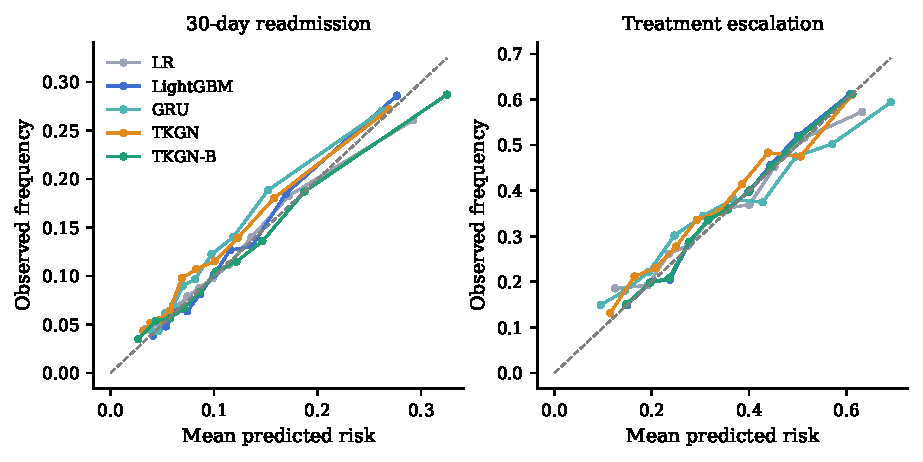
\includegraphics[width=\linewidth]{figures/fig_calibration.pdf}
  \caption{Reliability curves on the first grouped test set (ten
  equal-frequency bins).}
  \label{fig:calibration}
\end{figure}

\subsection{Statistical comparison}
Table~\ref{tab:significance} compares TKGN-B with every other model. Against
the deep sequence models, the advantage of TKGN-B was consistent and
statistically significant for readmission: it won all five repeats against
GRU, RETAIN, the Transformer and TKGN, and on the first test set the AUROC
difference to TKGN was \DaucReadmitTKGN{} (95\% CI \DaucLoReadmitTKGN{} to
\DaucHiReadmitTKGN{}; DeLong $p$ \PDelongReadmitTKGN{}). For escalation it
also won all five repeats against every sequence model (mean difference to
TKGN \RepDaucEscTKGN{}, paired $t$-test $p$ \RepPEscTKGN{}), although the
single-split bootstrap intervals, which are wider for this smaller task,
included zero.

Against the tuned gradient-boosting models the differences were small.
For readmission TKGN-B exceeded LightGBM in \WinsReadmitLGBM{} repeats
(mean $\Delta$AUROC \RepDaucReadmitLGBM{}, $p$ \RepPReadmitLGBM{}) and XGBoost
in \WinsReadmitXGB{} (mean \RepDaucReadmitXGB{}); for escalation it exceeded
both in \WinsEscLGBM{} repeats (mean \RepDaucEscLGBM{} and \RepDaucEscXGB{};
$p$ \RepPEscLGBM{} and \RepPEscXGB{}). None of these differences reached
significance on the first test set (bootstrap $p$ \PBootReadmitLGBM{} and
\PBootEscLGBM{} versus LightGBM). We therefore interpret TKGN-B as matching
the strongest tabular learners with a small but consistent advantage, not as
a decisive improvement over them.

\begin{table*}[t]
  \centering
  \caption{TKGN-B compared with each model. $\Delta$AUROC and its 95\%
  patient-clustered bootstrap CI refer to the first grouped test set;
  $p_\text{DeLong}$: DeLong test on the same set; Wins: repeats (of five)
  in which TKGN-B had the higher test AUROC; $p_\text{temp}$: DeLong test on
  the temporal test set (first seed). Positive values favour TKGN-B.}
  \label{tab:significance}
  \scriptsize
  \setlength{\tabcolsep}{3pt}
  \begin{tabular}{@{}l cccc cccc@{}}
\toprule
 & \multicolumn{4}{c}{30-day readmission} & \multicolumn{4}{c}{Treatment escalation} \\
\cmidrule(lr){2-5}\cmidrule(lr){6-9}
Comparator & $\Delta$AUROC [95\% CI] & $p_\text{DeLong}$ & Wins & $p_\text{temp}$ & $\Delta$AUROC [95\% CI] & $p_\text{DeLong}$ & Wins & $p_\text{temp}$ \\
\midrule
Logistic regression & +0.0224 [+0.0152, +0.0299] & $<$0.001 & 5/5 & $<$0.001 & +0.0240 [+0.0145, +0.0330] & $<$0.001 & 5/5 & $<$0.001 \\
Random forest & +0.0058 [-0.0004, +0.0114] & 0.055 & 5/5 & $<$0.001 & +0.0029 [-0.0020, +0.0076] & 0.237 & 5/5 & 0.003 \\
XGBoost & +0.0017 [-0.0028, +0.0063] & 0.472 & 4/5 & 0.001 & +0.0009 [-0.0025, +0.0045] & 0.593 & 5/5 & $<$0.001 \\
LightGBM & +0.0002 [-0.0037, +0.0038] & 0.901 & 4/5 & 0.159 & +0.0003 [-0.0004, +0.0011] & 0.359 & 5/5 & $<$0.001 \\
MLP & +0.0386 [+0.0297, +0.0472] & $<$0.001 & 5/5 & $<$0.001 & +0.0339 [+0.0227, +0.0450] & $<$0.001 & 5/5 & $<$0.001 \\
GRU & +0.0061 [+0.0004, +0.0115] & 0.028 & 5/5 & 0.087 & +0.0072 [-0.0010, +0.0156] & 0.120 & 5/5 & 0.001 \\
RETAIN & +0.0076 [+0.0017, +0.0132] & 0.006 & 5/5 & 0.405 & +0.0043 [-0.0048, +0.0134] & 0.367 & 5/5 & $<$0.001 \\
Transformer & +0.0104 [+0.0047, +0.0160] & $<$0.001 & 5/5 & 0.796 & +0.0026 [-0.0056, +0.0112] & 0.558 & 5/5 & 0.001 \\
TKGN (proposed) & +0.0111 [+0.0060, +0.0161] & $<$0.001 & 5/5 & 0.562 & +0.0045 [-0.0047, +0.0136] & 0.332 & 5/5 & 0.011 \\
\bottomrule
\end{tabular}

\end{table*}

\subsection{Temporal validation and dataset shift}
The temporal split tests models on the most recent admissions after
fitting them on older ones. For treatment escalation TKGN-B was again the
best model (AUROC \AucEscTmpTKGNB{} versus \AucEscTmpXGB{} for XGBoost and
\AucEscTmpLGBM{} for LightGBM), and on the first seed its advantage was
significant against every comparator (e.g.\ $\Delta$AUROC \DaucTmpEscLGBM{}
versus LightGBM, DeLong $p$ \PDelongTmpEscLGBM{}). For readmission the
picture differed: random forest achieved the highest AUROC
(\AucReadmitTmpRF{}), while TKGN-B (\AucReadmitTmpTKGNB{}), LightGBM
(\AucReadmitTmpLGBM{}) and XGBoost (\AucReadmitTmpXGB{}) were close to each
other and TKGN alone reached \AucReadmitTmpTKGN{}.

The temporal test period differs markedly from the training period. The
maximum number of recorded diagnoses per stay rose from \ShiftTrainDxMax{}
to \ShiftTestDxMax{} (mean \ShiftTrainDxMean{} versus \ShiftTestDxMean{}),
the share of stays preceded by an earlier stay rose from
\ShiftTrainHist\% to \ShiftTestHist\%, the longest history grew from
\ShiftTrainMaxPrior{} to \ShiftTestMaxPrior{} earlier stays, and emergency
visits in the prior year nearly doubled (\ShiftTrainEmerg{} versus
\ShiftTestEmerg{}). Models that extrapolate linearly suffered most:
logistic regression fell to an AUROC of \AucReadmitTmpLR{} with a
calibration slope of \SlopeReadmitTmpLR{}, and the MLP to
\AucReadmitTmpMLP{}. Tree ensembles, whose predictions are bounded outside
the training range, and sequence models, which bound history through a fixed
window and learned summaries, were much more robust.

\subsection{Ablation}
Table~\ref{tab:ablation} and Fig.~\ref{fig:ablation} show the effect of
removing each TKGN component (first \NAblRuns{} grouped repeats). Access to
earlier encounters was by far the most important element: without it,
AUROC dropped by \AblReadmitTnohistory{} for readmission and
\AblEscTnohistory{} for escalation. Removing the outcomes of earlier stays
or the auxiliary outcome head reduced readmission AUROC by
\AblReadmitTnoprioroutcomes{} and \AblReadmitTnoaux{}, but not escalation
AUROC. The history-reliability gates and the delta encoding had effects
within $\pm$0.001, i.e.\ within run-to-run variation. Contrary to our
expectation, the knowledge-graph components did not help with the full
training set: flat code embeddings changed AUROC by \AblReadmitTnokg{}
(readmission) and \AblEscTnokg{} (escalation), and removing only the
co-morbidity propagation gave \AblReadmitTnocooccurrence{} and
\AblEscTnocooccurrence{}, i.e.\ the hierarchy-only variant was the best
TKGN configuration on test data. Because this was observed after the design
had been fixed on validation data, we report the pre-specified
configuration as TKGN and treat the hierarchy-only variant as a finding to be
confirmed in future work.

\begin{table}[t]
  \centering
  \caption{Ablation of TKGN (mean$\pm$SD test AUROC over the first
  \NAblRuns{} grouped repeats; $\Delta$ relative to the full model).}
  \label{tab:ablation}
  \scriptsize
  \setlength{\tabcolsep}{3pt}
  \begin{tabular}{@{}lcccc@{}}
\toprule
 & \multicolumn{2}{c}{30-day readmission} & \multicolumn{2}{c}{Treatment escalation} \\
\cmidrule(lr){2-3}\cmidrule(lr){4-5}
Variant & AUROC & $\Delta$ & AUROC & $\Delta$ \\
\midrule
Full TKGN & 0.6847$\pm$0.0035 & -- & 0.6781$\pm$0.0151 & -- \\
$-$ knowledge graph (flat code embeddings) & 0.6857$\pm$0.0038 & +0.0011 & 0.6819$\pm$0.0172 & +0.0038 \\
$-$ co-morbidity (PPMI) propagation & 0.6888$\pm$0.0036 & +0.0042 & 0.6843$\pm$0.0162 & +0.0063 \\
$-$ earlier encounters (index stay only) & 0.6773$\pm$0.0059 & -0.0073 & 0.6601$\pm$0.0191 & -0.0179 \\
$-$ history-reliability gates & 0.6837$\pm$0.0036 & -0.0009 & 0.6778$\pm$0.0158 & -0.0002 \\
$-$ delta encoding & 0.6851$\pm$0.0038 & +0.0005 & 0.6770$\pm$0.0137 & -0.0010 \\
$-$ outcomes of earlier stays & 0.6826$\pm$0.0033 & -0.0021 & 0.6803$\pm$0.0156 & +0.0023 \\
$-$ auxiliary outcome head & 0.6826$\pm$0.0025 & -0.0021 & 0.6819$\pm$0.0202 & +0.0039 \\
\bottomrule
\end{tabular}

\end{table}

\begin{figure}[t]
  \centering
  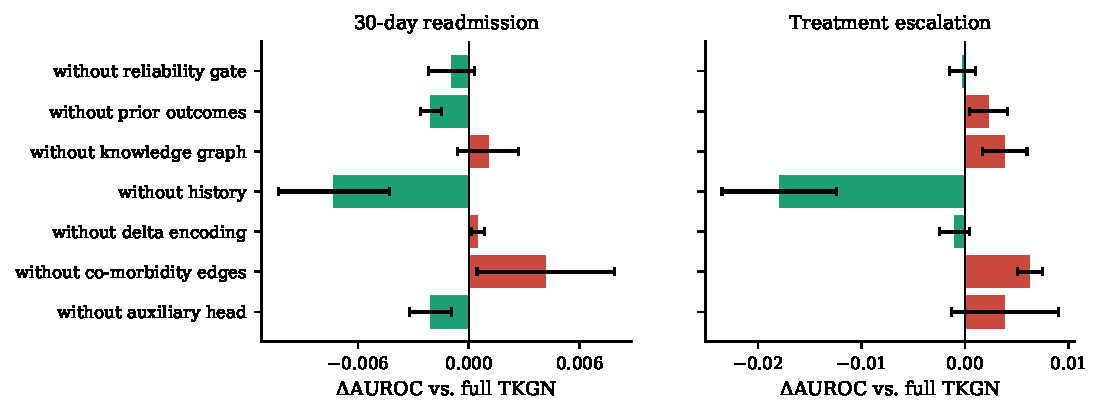
\includegraphics[width=\linewidth]{figures/fig_ablation.pdf}
  \caption{Change in test AUROC when one component of TKGN is removed
  (mean$\pm$SD of paired differences over repeats). Green: the component
  helps; red: the model is better without it.}
  \label{fig:ablation}
\end{figure}

\subsection{Knowledge graph under data scarcity}
\label{sec:kgeff}
Because ontology-based representations are expected to help most when
training data are limited, we retrained TKGN with and without the knowledge
graph on 5, 10 and 25\% of the training patients in three grouped repeats,
with identical patient subsets and seeds for both variants
(Table~\ref{tab:kg}). The hypothesis was not supported. For readmission the
paired differences were close to zero at every size (\KgReadmitFive{},
\KgReadmitTen{} and \KgReadmitTwentyFive{} AUROC at 5, 10 and 25\%), with
standard deviations several times larger than the means. For escalation the
flat-embedding variant was never worse on average (\KgEscFive{},
\KgEscTen{} and \KgEscTwentyFive{}). On this cohort, whose diagnosis codes
are mostly truncated to three characters, sharing information along the
ICD-9-CM hierarchy and the co-morbidity graph therefore did not improve
discrimination at any training-set size we examined.

\begin{table}[t]
  \centering
  \caption{TKGN with and without the knowledge graph (KG) trained on subsets
  of the training patients. Mean test AUROC over three grouped repeats with
  paired subsets and seeds; $\Delta$ = TKGN minus TKGN without KG; Wins:
  repeats in which the KG variant was better.}
  \label{tab:kg}
  \scriptsize
  \setlength{\tabcolsep}{3pt}
  \begin{tabular}{@{}llcccc@{}}
\toprule
Task & Training share & TKGN & TKGN $-$ KG & $\Delta$AUROC (mean$\pm$SD) & Wins \\
\midrule
30-day readmission & 5\% & 0.6387 & 0.6395 & -0.0009$\pm$0.0063 & 1/3 \\
 & 10\% & 0.6495 & 0.6487 & +0.0008$\pm$0.0054 & 2/3 \\
 & 25\% & 0.6717 & 0.6715 & +0.0003$\pm$0.0049 & 2/3 \\
 & 100\% & 0.6847 & 0.6857 & -0.0011$\pm$0.0017 & 0/3 \\
\midrule
Treatment escalation & 5\% & 0.6049 & 0.6201 & -0.0152$\pm$0.0205 & 1/3 \\
 & 10\% & 0.6331 & 0.6336 & -0.0005$\pm$0.0031 & 1/3 \\
 & 25\% & 0.6585 & 0.6596 & -0.0012$\pm$0.0030 & 1/3 \\
 & 100\% & 0.6781 & 0.6819 & -0.0038$\pm$0.0021 & 0/3 \\
\bottomrule
\end{tabular}

\end{table}


\subsection{Data efficiency}
Fig.~\ref{fig:learning} and Table~\ref{tab:learning} show performance when
only part of the training patients is available. TKGN-B was at least as
good as LightGBM at every training size for readmission, with the largest
gains at small sizes (5\%: \LcReadmitFiveTKGNB{} versus
\LcReadmitFiveLGBM{}; 25\%: \LcReadmitTwentyFiveTKGNB{} versus
\LcReadmitTwentyFiveLGBM{}). For escalation, LightGBM was better with 5\% of
the training patients (\LcEscFiveLGBM{} versus \LcEscFiveTKGNB{}) and
TKGN-B was better from 10\% onwards (e.g.\ 50\%: \LcEscFiftyTKGNB{} versus
\LcEscFiftyLGBM{}). These curves come from one repeat each and should be
read as trends.

\begin{figure}[t]
  \centering
  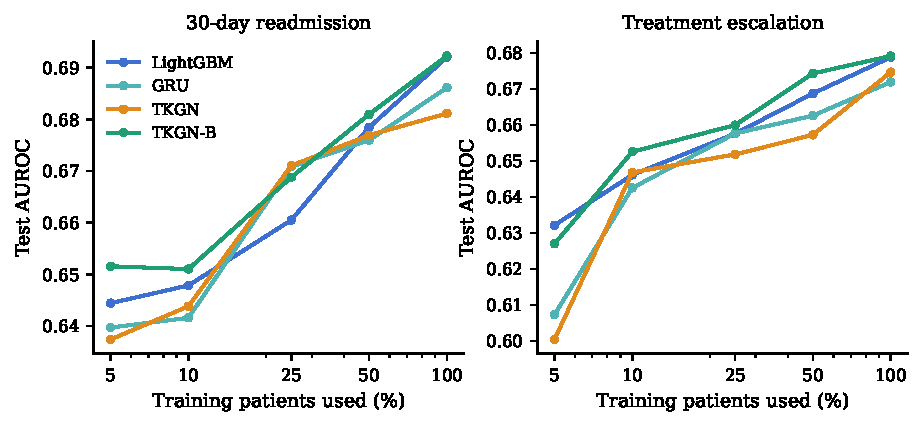
\includegraphics[width=\linewidth]{figures/fig_learning_curve.pdf}
  \caption{Test AUROC as a function of the share of training patients
  (first grouped repeat; same test patients at every size).}
  \label{fig:learning}
\end{figure}

\begin{table}[t]
  \centering
  \caption{Learning curve: test AUROC by share of training patients.}
  \label{tab:learning}
  \scriptsize
  \begin{tabular}{@{}llccccc@{}}
\toprule
Task & Model & 5\% & 10\% & 25\% & 50\% & 100\% \\
\midrule
30-day readmission & LightGBM & 0.644 & 0.648 & 0.660 & 0.678 & 0.692 \\
 & GRU & 0.640 & 0.642 & 0.671 & 0.676 & 0.686 \\
 & TKGN & 0.637 & 0.644 & 0.671 & 0.677 & 0.681 \\
 & TKGN-B & 0.652 & 0.651 & 0.669 & 0.681 & 0.692 \\
\midrule
Treatment escalation & LightGBM & 0.632 & 0.646 & 0.658 & 0.669 & 0.679 \\
 & GRU & 0.607 & 0.643 & 0.658 & 0.663 & 0.672 \\
 & TKGN & 0.600 & 0.647 & 0.652 & 0.657 & 0.675 \\
 & TKGN-B & 0.627 & 0.653 & 0.660 & 0.674 & 0.679 \\
\bottomrule
\end{tabular}

\end{table}

\subsection{Patients with and without earlier stays}
For readmission, discrimination was lower for patients with a longer
history, whose baseline risk is higher and more homogeneous
(Table~\ref{tab:subgroups}); for escalation it was higher
(\SubEscZeroTKGNB{} for first stays versus \SubEscTwoTKGNB{} with two or
more earlier stays). For readmission among patients with two or more earlier stays, TKGN-B reached
an AUROC of \SubReadmitTwoTKGNB{}, compared with \SubReadmitTwoLGBM{} for
LightGBM, and TKGN alone reached \SubReadmitTwoTKGN{}; the sequence
information therefore contributes most where the tabular history summaries
saturate. For first stays the two approaches were equivalent
(\SubReadmitZeroTKGNB{} versus \SubReadmitZeroLGBM{}).

The learned gates behaved differently for the two tasks
(Fig.~\ref{fig:gates}). For escalation, the mean history gate increased with
the number of earlier stays (\GateEscZero{} with none, \GateEscFive{} with
five or more), i.e.\ the model relied more on longer histories. For
readmission, the gate was lower for patients with history than the value
it applied to the learned ``no history'' vector (\GateReadmitOne{} with one
earlier stay, \GateReadmitZero{} with none), indicating that the network
damped the history summary and relied on the index stay together with the
outcome tokens of earlier stays.

\begin{figure}[t]
  \centering
  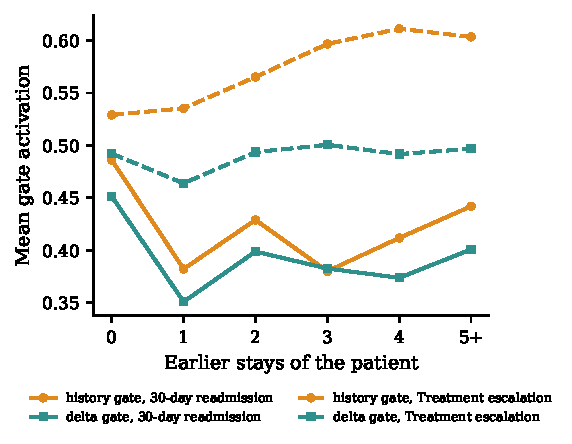
\includegraphics[width=0.62\linewidth]{figures/fig_gates.pdf}
  \caption{Mean activation of the history and delta gates by number of
  earlier stays (first grouped test set).}
  \label{fig:gates}
\end{figure}

\subsection{Explanations}
Permutation importance (Fig.~\ref{fig:importance}) identified
\TopGroupReadmit{} as the most important input group of TKGN for
readmission (AUROC drop \TopGroupDropReadmit{}), followed by the sequence of
earlier encounters and the admission and discharge context; for escalation
the anti-diabetic medication profile dominated (drop
\TopGroupDropEsc{}), again followed by earlier encounters. HbA1c and glucose
results contributed almost nothing, consistent with the fact that they were
measured in fewer than one in five stays. For the LightGBM anchor, TreeSHAP
ranked the number of inpatient stays in the preceding year and discharge
home as the strongest readmission predictors, and a steady insulin dose and
the change in the number of prescribed diabetes drugs since the last stay as
the strongest escalation predictors. These patterns agree with clinical
knowledge on readmission after diabetes admissions \citep{rubin2015} and
support the plausibility of the models.

\begin{figure*}[t]
  \centering
  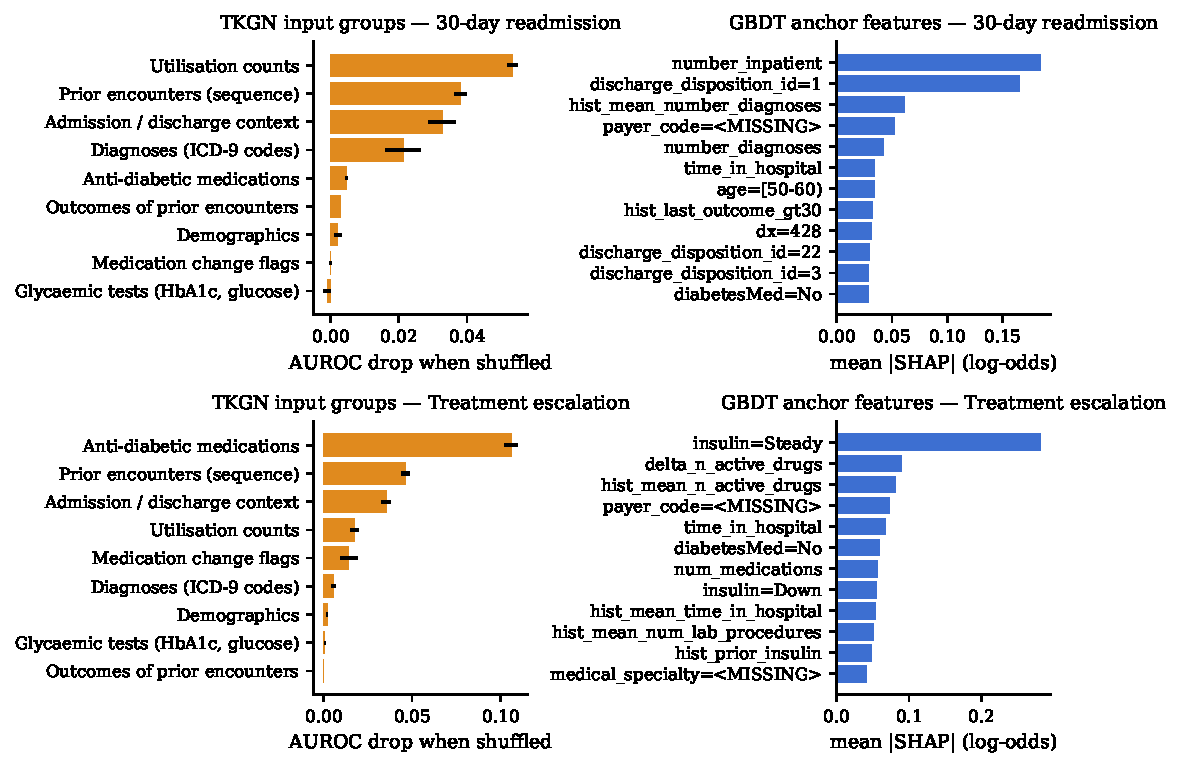
\includegraphics[width=\textwidth]{figures/fig_importance.pdf}
  \caption{Left: permutation importance of input groups for TKGN (mean AUROC
  drop over three permutations). Right: mean absolute TreeSHAP value of the
  LightGBM anchor of TKGN-B. First grouped test set.}
  \label{fig:importance}
\end{figure*}

\subsection{Subgroups and fairness}
Table~\ref{tab:subgroups} and Fig.~\ref{fig:subgroups} report subgroup
performance. For readmission, the AUROC of TKGN-B differed by at most
\GapReadmitRace{} between racial groups with at least 300 test encounters
(African American \SubRaceReadmitAA{}, Caucasian \SubRaceReadmitCA{}), by
\GapReadmitGender{} between women and men, and by \GapReadmitAge{} between
age bands, with the lowest discrimination in patients aged 70 years or older.
For escalation the corresponding gaps were \GapEscRace{}, \GapEscGender{} and
\GapEscAge{}. Calibration within subgroups was acceptable (ECE at most
\MaxSubEce{} in all groups with at least 300 encounters). Groups
with fewer than 300 test encounters (Asian, $n=105$) give unstable
estimates and are shown for completeness only.

\begin{table}[t]
  \centering
  \caption{Test AUROC by subgroup (first grouped repeat).}
  \label{tab:subgroups}
  \scriptsize
  \setlength{\tabcolsep}{3pt}
  \begin{tabular}{@{}lcccccc@{}}
\toprule
 & \multicolumn{3}{c}{30-day readmission} & \multicolumn{3}{c}{Treatment escalation} \\
\cmidrule(lr){2-4}\cmidrule(lr){5-7}
Subgroup & $n$ & TKGN-B & LightGBM & $n$ & TKGN-B & LightGBM \\
\midrule
\multicolumn{7}{@{}l}{\textit{Race}} \\
\quad AfricanAmerican & 3,707 & 0.715 & 0.713 & 1,256 & 0.695 & 0.695 \\
\quad Asian & 105 & 0.802 & 0.768 & -- & -- & -- \\
\quad Caucasian & 14,783 & 0.684 & 0.684 & 4,260 & 0.669 & 0.669 \\
\quad Hispanic & 424 & 0.693 & 0.687 & -- & -- & -- \\
\quad Other & 316 & 0.736 & 0.727 & -- & -- & -- \\
\quad Unknown & 459 & 0.718 & 0.733 & -- & -- & -- \\
\multicolumn{7}{@{}l}{\textit{Gender}} \\
\quad Female & 10,560 & 0.703 & 0.704 & 3,230 & 0.679 & 0.678 \\
\quad Male & 9,234 & 0.680 & 0.678 & 2,539 & 0.679 & 0.679 \\
\multicolumn{7}{@{}l}{\textit{Age (years)}} \\
\quad 50-69 & 7,830 & 0.693 & 0.694 & 2,293 & 0.684 & 0.683 \\
\quad 70+ & 8,736 & 0.660 & 0.659 & 2,595 & 0.682 & 0.682 \\
\quad <50 & 3,228 & 0.758 & 0.756 & 881 & 0.660 & 0.659 \\
\multicolumn{7}{@{}l}{\textit{Earlier stays}} \\
\quad 0 & 13,998 & 0.673 & 0.671 & 3,268 & 0.667 & 0.667 \\
\quad 1 & 3,271 & 0.665 & 0.662 & 1,188 & 0.696 & 0.695 \\
\quad 2+ & 2,525 & 0.620 & 0.608 & 1,313 & 0.693 & 0.692 \\
\multicolumn{7}{@{}l}{\textit{HbA1c}} \\
\quad measured & 3,387 & 0.675 & 0.681 & 914 & 0.705 & 0.704 \\
\quad not measured & 16,407 & 0.695 & 0.693 & 4,855 & 0.674 & 0.674 \\
\bottomrule
\end{tabular}

\end{table}

\begin{figure*}[t]
  \centering
  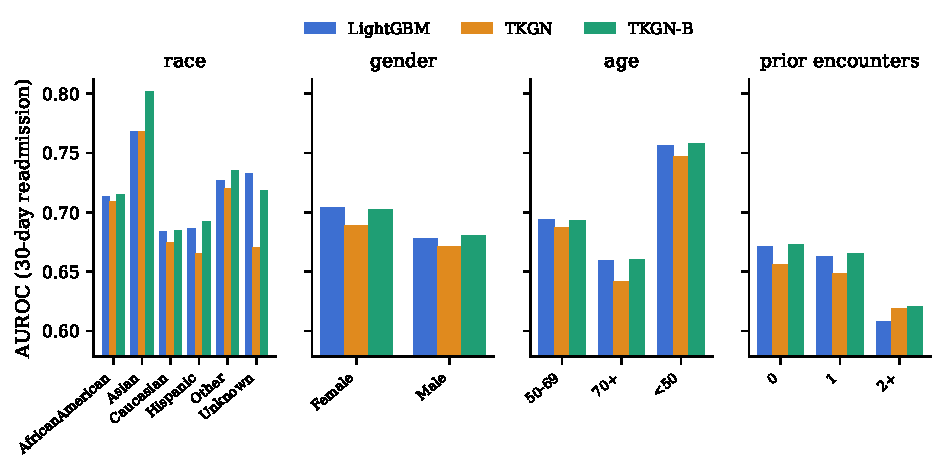
\includegraphics[width=\textwidth]{figures/fig_subgroups.pdf}
  \caption{30-day readmission AUROC by race, sex, age band and number of
  earlier stays.}
  \label{fig:subgroups}
\end{figure*}
